\documentclass[12pt]{report}

\title{Decentralised location proof system}

\usepackage[utf8]{inputenc}
\usepackage{graphicx}
\usepackage{subcaption}

\usepackage{tikz}
\usetikzlibrary{calc,arrows}
\usepackage{enumitem}
\usepackage{float}
\usepackage{subfig}

\author{Conor Taylor}
\date{
	B.A.(Mod.) Computer Science\\
	Final Year Project, April 2016\\
	Supervisor: Stephen Barrett
}

\begin{document}
\maketitle

\tableofcontents
\newpage

\listoffigures
\newpage

\chapter{Introduction}
\section{Project and Motivation}
Location verification is the process of verifying whether a \textit{node} (computer) is physically present at a location it claims to be. Existing location proof systems attept to use centralised, trusted ``authoritive'' nodes to provide proof of another node's location. These approaches require investment in infrastructure, and are subject to privacy violation and denial of service attacks. This project aims to present a \textit{decentralised} solution to this problem. A decentralised location proof system is a system in which there is no ``authoritive source'' trusted and relied upon to provide and store sensitive location information.

This project describes a decentralised location proof system that is capable of operating on \textit{mobile nodes} (mobile devices). I propose a design in which location proofs are obtained using other untrusted mobile nodes as \textit{alibi's}. Proofs will be created as two mobile nodes communicate over an ad-hoc bluetooth network, transfer encrypted location information, and publish it on a public append-only bulletin board, known as a \textit{blockchain}. The decentralised nature of the system means that there is no single point of failure, no entity controlling the security of every node's location proofs, and no entity capable of violating another node's privacy. This is because in a decentralised system, no node is ``in charge'', and no node has more authority in the system than any other node.

\chapter{Background}
\section{Background}
\subsection{Proving your location}
As an increasing amount of personal information is accessible on the internet and therefore on mobile devices, the security that existed by requiring physical interaction between humans to transfer sensitive data is lost.

\subsection{Ad-hoc networks}

\subsection{Blockchain}

\subsection{Centralised location proof systems}
Location proof systems are expected to be accurate and tamper-proof. For this reason, existing solutions have chosen to use a central authority to issue proofs, or to regulate proof issuance \cite{brassil, luo, khan}.

A hardware technique \cite{brassil} operates by supplementing existing WiFi access points with \textit{femtocells}. A femtocell is a small cellular antenna that connects to a mobile carrier via the Internet. Location verification over the internet is made possible by determining which femtocell a mobile node is connected to as it transfers data via Wi-Fi. This solution requires investment in additional hardware to supplement existing WiFi access points, and requires access to mobile providers' user database to identify users locations.

The use of a centralised system, like that described by Brassil et al. \cite{brassil}, creates security, privacy and vulnerability issues. An attacker who succeeds in compromising the security of the central server can violate the privacy of the users of the system, and potentially track their location. The central system architecture is also vulnerable, in the sense that a resource availability attack such as a DDoS attack could render the central architecture unavailable, making location verification unavailable.

Luo et al. propose a system that uses Wi-Fi access points (\textit{AP's}) to allow users to create location proofs \cite{luo}. In their system, each access point has a \textit{group signature} and can sign location proofs for requesting users. Users can request a location proof from any access point, and receive a proof encrypted by the AP with the group signature, as shown in figure \ref{fig:luo_transaction}. This can then be submitted to a Verifier.

\begin{figure}[H]
\begin{center}
\resizebox {0.6\columnwidth} {!} {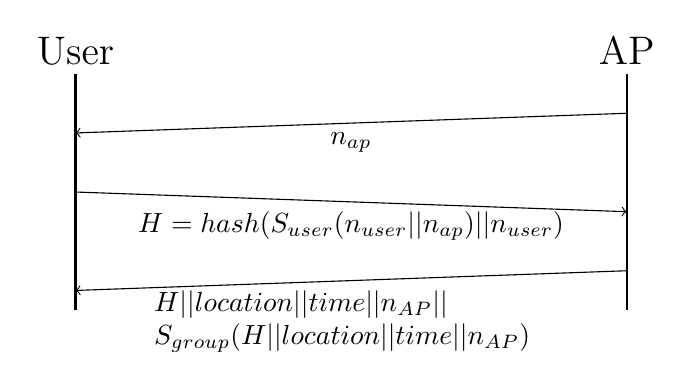
\begin{tikzpicture}
\coordinate (A_T) at (0,3);
\coordinate (A_B) at (0,0);
\coordinate (A_1) at (0,2.25);
\coordinate (A_2) at (0,1.5);
\coordinate (A_3) at (0,0.25);

\coordinate (B_T) at (7,3);
\coordinate (B_B) at (7,0);
\coordinate (B_1) at (7,2.5);
\coordinate (B_2) at (7,1.25);
\coordinate (B_3) at (7,0.5);

\draw[thick] (A_T)--(A_B);
\draw[thick] (B_T)--(B_B);
\draw (A_T) node[above]{\Large User};
\draw (B_T) node[above]{\Large AP};

\draw[->] (B_1) -- (A_1) node[midway,below] {$n_{ap}$};
\draw[->] (A_2) -- (B_2) node[midway,below]
	{$H = hash(S_{user}(n_{user} || n_{ap}) || n_{user})$};
	
\draw[->] (B_3) -- (A_3) node[text width=5cm,midway,below]
	{$H || location || time || n_{AP} ||$\\
	$S_{group}(H || location || time || n_{AP})$};
\end{tikzpicture}}
\end{center}
\caption{Adopted from Luo et al. \cite{luo}}
\label{fig:luo_transaction}
\end{figure}

This kind of system creates \textit{proactive} location proofs. A proactive location proof is one which is created before it is needed. The user creates application-independent location proofs, and can use them at a later time with any application(s) he chooses.

\chapter{Design}
The location proof system I propose allows \textit{mobile nodes} to create location proofs by initiating an \textit{exchange} with another anonymous mobile node. When two mobile nodes are in close physical proximity, they initiate an exchange in the background over a short range, ad-hoc network such as Bluetooth. On completion of the exchange, both nodes can generate their own \textit{transaction}, a cryptographically secure proof of location, attested by the other mobile node.

To create a transaction, two mobile nodes anonymously exchange their GPS coordinates and current time over the ad-hoc network. Both nodes then check that these parameters don't differ from their own observed parameters by more than some value $\epsilon$. Once satisfied, they each create an encrypted, privacy-protecting transaction logging their location and the identity of the other mobile node (the \textit{alibi}) used to create the transaction. This transaction is published onto a public, append-only bulletin board known as a \textit{blockchain} \cite{blueprint}. Once given permission from a mobile node, a \textit{Verifier node} can consult the data in blockchain and determine whether or not the mobile node is present at its claimed location.

Any mobile node acting as an alibi in a transaction will share details of its most recent transactions with the other mobile node in the exchange. This means that when the mobile node seeks verification from a Verifier node, the Verifier can examine the mobile node's alibi's, and each of the alibi's recent alibi's, forming a large tree of connections which can be used to verify or reject the mobile nodes claimed location. Only the owner of the transaction can give permission to a Verifier to check its location history, by providing the Verifier with the keys needed to decrypt the transactions.

Figure \ref{fig:overview} provides an overview of the operation of the proposed system.

\begin{figure}[H]
\begin{center}
\resizebox {\columnwidth} {!} {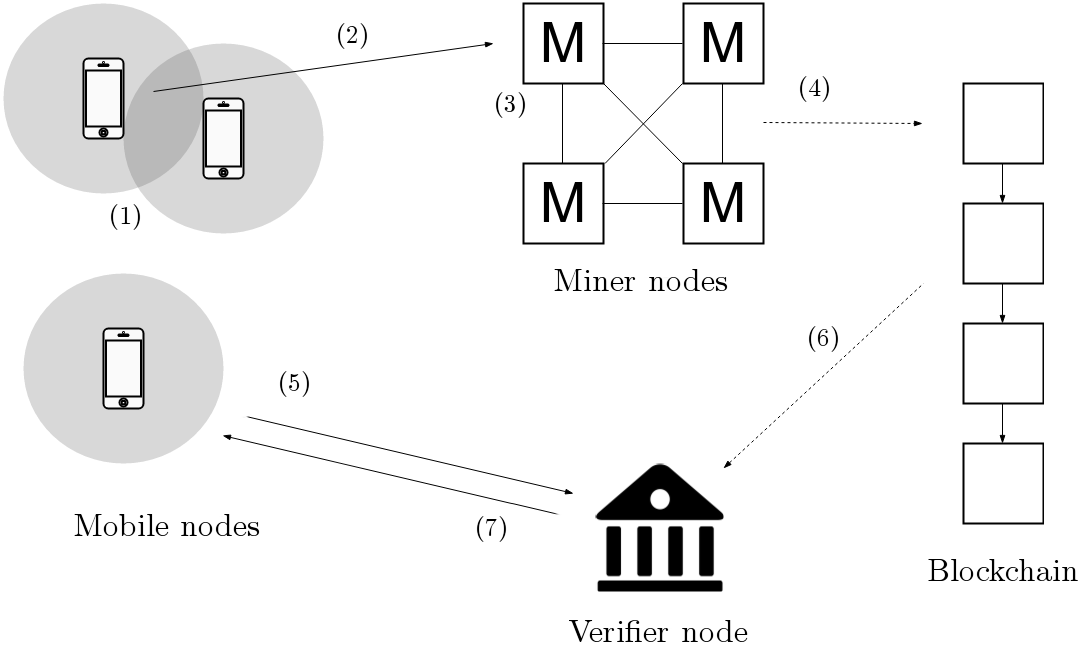
\includegraphics{diagrams/overview.png}}
\caption{Design and operation overview}
\label{fig:overview}
\end{center}
\end{figure}

\begin{enumerate}[label=\textbf{\arabic*}.]
\item Two mobile nodes come in close physical proximity and create an ad-hoc network, over which they initiate an exchange and each create a transaction.
\item Both mobile nodes publish their own transaction to a Miner node.
\item The Miner node who received the transaction distributes it across the Miner network.
\item One Miner node solves the proof-of-work for a block of transactions, and the new block is appended to the blockchain.
\item A mobile node requests verification from a Verifier node (request structure is explained in section \ref{ssec:verification}).
\item The Verifier node uses the public blockchain to examine the requesting node's transactions and determine their validity.
\item The Verifier accepts or rejects the  mobile node's claimed location based on its analysis of the transactions in the blockchain. 
\end{enumerate}

\section{Identities}
In order to preserve user's privacy, a user will only ever use an identity for one transaction, before generating a new one. This prevents curious users from watching the public blockchain for a known identity and tracking it. However, to prevent identity theft, it is important for the Verifier to be able to prove that a mobile node is the owner of each identity. This is achieved using a public/private key pair for each mobile node.

When a mobile node is first joins the network, it generates a public/private key pair. To maintain anonymity, the mobile node will use the public key to encrypt \textit{nonces} to create \textit{identities}, and use these to identify itself in a transaction. A different identity will be created for each transaction. During the verification stage, the node will provide the Verifier with its public key, along with the list of the nonces used to generate its $n$ most recent transactions (see figure \ref{fig:verify_request}). This allows the Verifier to calculate all of the node's identities, and prove that they were all created by the same node. The Verifier can then retrieve the transactions associated with those identities from the blockchain. The Verifier will also ensure that the node owns the private key associated with the provided public key, to prevent a weak identity attack.

\subsection{Nonce list} \label{sssec:nonce_list}
A \textit{Nonce List} is simply a list of all of the nonces a mobile node has used so far to generate identities. When a mobile node wishes to generate a new identity, it must first generate a new nonce which is then encrypted to create the identity. The nonce is appended to the mobile node's nonce list, so it can be used later during verification (see section \ref{ssec:verification}).

\begin{figure}[H]
\resizebox {\columnwidth} {!} {\documentclass[border=2pt]{standalone}
\usepackage{tikz}
\usetikzlibrary{matrix,positioning,arrows.meta,arrows,calc}

\tikzset{
mymat/.style={
  matrix of math nodes,
  text height=2.5ex,
  text depth=0.75ex,
  text width=5.25ex,
  align=center,
  column sep=-\pgflinewidth
  },
mymats/.style={
  mymat,
  text width=8ex,
  nodes={draw}
  }  
}
\begin{document}

\begin{tikzpicture}[>=latex]
\matrix[mymat,anchor=west,row 1/.style={nodes=draw}]
at (0,0) 
(mat1)
{
4827 & 1928 & 9183 & 0047\\
};
\matrix[mymats=white,anchor=west]
at (0,-3) 
(mat3)
{
12ef5a1 & c100e9d & 038ef6b & ee3bc14 \\
};

\node[left=0pt of mat1]
  (cella) {Nonce list:};
  
\node[left=0pt of mat3]
  (cella) {Identities:};
  
  
\node (key) at ($(mat1-1-4.south)!0.5!(mat3-1-4.north)$) {$K^+(0047)$};

\begin{scope}[shorten <= -2pt]
\draw[*->]
  (mat1-1-1.south) -- (mat3-1-1.north);
\draw[*->]
  (mat1-1-2.south) -- (mat3-1-2.north);
\draw[*->]
  (mat1-1-3.south) -- (mat3-1-3.north);
\draw[*-]
  (mat1-1-4.south) -- (key);
\draw[->]
  (key) -- (mat3-1-4.north);
\end{scope}
\end{tikzpicture}

\end{document}}
\caption{Identity generation from Nonce List}
\label{fig:nonce_list}
\end{figure}

In figure \ref{fig:nonce_list} above, nonce $0047$ is encrypted with $K^+$ to create identity $ee3bc14$. By providing the nonce list and $K^+$, a node can prove that it created all of the identities in the identities list. It must also verify that it owns $K^-$, its private key.

\subsection{Identity duplication}
Since all identities are generated from random nonces, there is nothing to prevent two nodes from generating the same identity and using it in different transactions. It is therefore possible that during verification, a Verifier node may find multiple transactions with the same ID while searching the blockchain. The Verifier will have a decryption key for the transaction it is searching for, which will only successfully decrypt one of the transactions with the duplicate ID. The Verifier will try to decrypt each one until it finds the one that can be decrypted successfully.

\newpage
\section{Transactions} \label{sec:transactions}
During an exchange between two nodes, a number of different items must be shared and calculated. Figure \ref{fig:transaction} describes and explains an honest, successful exchange, assuming an ad-hoc Bluetooth network has already been set up between nodes $A$ and $B$.

\begin{figure}[H]
\begin{center}
\resizebox {1.1\columnwidth} {!} {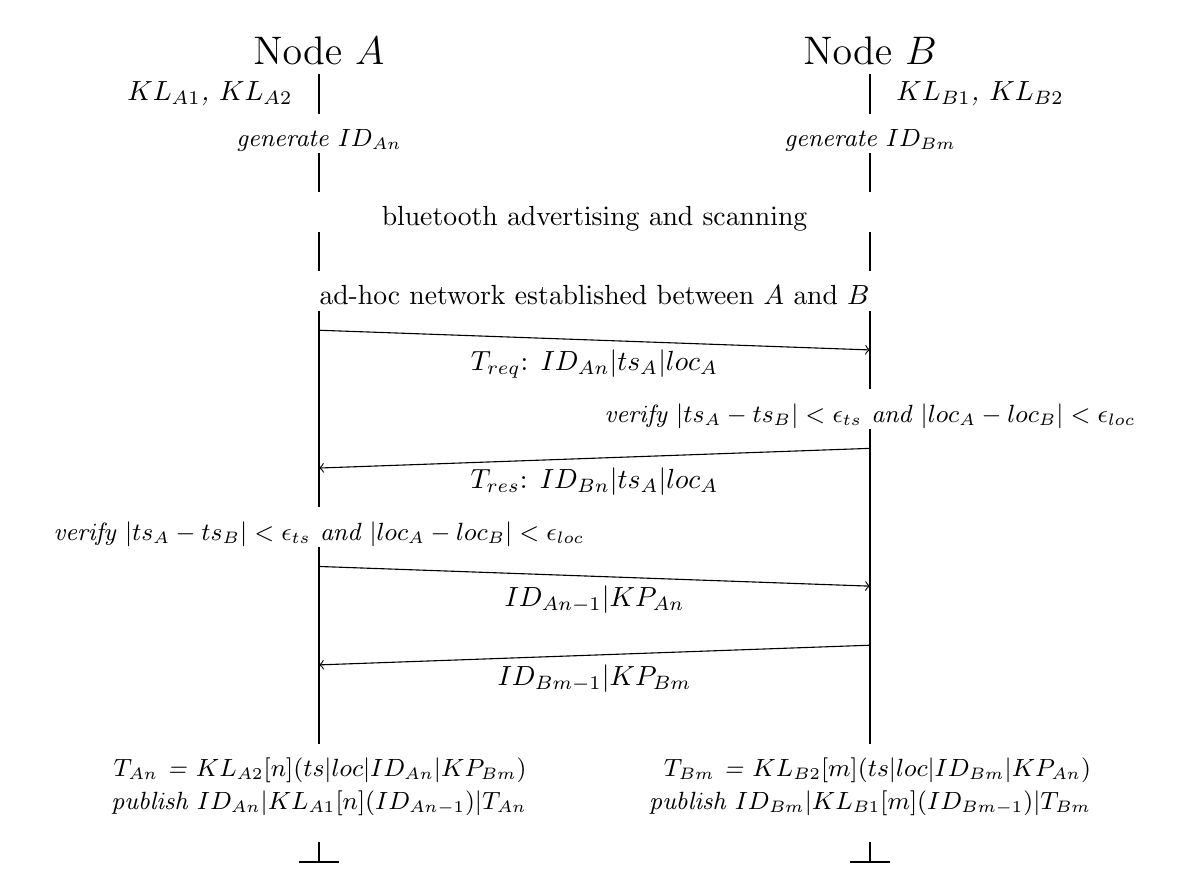
\begin{tikzpicture}
\coordinate (A_1) at (0,10);
\coordinate (A_2) at (0,9.5);
\coordinate (A_3) at (0,9);
\coordinate (A_4) at (0,8.5);
\coordinate (A_5) at (0,8);
\coordinate (A_6) at (0,7.5);
\coordinate (A_7) at (0,7);
\coordinate (A_8) at (0,4.5);
\coordinate (A_9) at (0,4);
\coordinate (A_10) at (0,1.5);
\coordinate (A_11) at (0,0.25);
\coordinate (A_12) at (0,0);
\coordinate (AF_L) at (-0.25,0);
\coordinate (AF_R) at (0.25,0);

\coordinate (M_1) at (3.5,8.5);
\coordinate (M_2) at (3.5,7.5);

\coordinate (B_1) at (7,10);
\coordinate (B_2) at (7,9.5);
\coordinate (B_3) at (7,9);
\coordinate (B_4) at (7,8.5);
\coordinate (B_5) at (7,8);
\coordinate (B_6) at (7,7.5);
\coordinate (B_7) at (7,7);
\coordinate (B_8) at (7,6);
\coordinate (B_9) at (7,5.5);
\coordinate (B_10) at (7,1.5);
\coordinate (B_11) at (7,0.25);
\coordinate (B_12) at (7,0);
\coordinate (BF_L) at (6.75,0);
\coordinate (BF_R) at (7.25,0);

\draw[thick] (A_1)--(A_2) (A_3)--(A_4) (A_5)--(A_6) (A_7)--(A_8) (A_9)--(A_10) (A_11)--(A_12) (AF_L)--(AF_R);
\draw[thick] (B_1)--(B_2) (B_3)--(B_4) (B_5)--(B_6) (B_7)--(B_8) (B_9)--(B_10) (B_11)--(B_12) (BF_L)--(BF_R);
\draw (A_1) node[above]{\Large Node $A$};
\draw (B_1) node[above]{\Large Node $B$};

\draw ($(A_1)!.5!(A_2)$) node[left]{\begin{tabular}{r}
\textit{$KL_{A1}$, $KL_{A2}$}
\end{tabular}};

\draw ($(B_1)!.5!(B_2)$) node[right]{\begin{tabular}{r}
\textit{$KL_{B1}$, $KL_{B2}$}
\end{tabular}};

\draw (A_2) node[below,text centered]{\begin{tabular}{r}
\small{\textit{generate $ID_{An}$}}
\end{tabular}};

\draw (B_2) node[below,text centered]{\begin{tabular}{r}
\small{\textit{generate $ID_{Bm}$}}
\end{tabular}};

\draw (M_1) node[below,text centered]{\begin{tabular}{r}
bluetooth advertising and scanning
\end{tabular}};

\draw (M_2) node[below,text centered]{\begin{tabular}{r}
ad-hoc network established between $A$ and $B$
\end{tabular}};

\coordinate (AX_1) at ($(A_7)-(0,0.25)$);
\coordinate (BX_1) at ($(B_7)-(0,0.5)$);
\draw[->] (AX_1) -- (BX_1) node[midway,below]
	{$T_{req}$: $ID_{An} | ts_A | loc_A$};
	
\draw (B_8) node[below,text centered]{\begin{tabular}{r}
\small{\textit{verify $|ts_A-ts_B| < \epsilon_{ts}$ and $|loc_A-loc_B| < \epsilon_{loc}$}}
\end{tabular}};

\coordinate (AX_2) at ($(A_7)-(0,2)$);
\coordinate (BX_2) at ($(B_9)-(0,0.25)$);
\draw[->] (BX_2) -- (AX_2) node[midway,below]
	{$T_{res}$: $ID_{Bn} | ts_A | loc_A$};
	
\draw (A_8) node[below,text centered]{\begin{tabular}{r}
\small{\textit{verify $|ts_A-ts_B| < \epsilon_{ts}$ and $|loc_A-loc_B| < \epsilon_{loc}$}}
\end{tabular}};

\coordinate (AX_3) at ($(A_9)-(0,0.25)$);
\coordinate (BX_3) at ($(B_9)-(0,2)$);
\draw[->] (AX_3) -- (BX_3) node[midway,below]
	{$ID_{An-1}|KP_{An}$};

\coordinate (AX_4) at ($(A_9)-(0,1.5)$);
\coordinate (BX_4) at ($(B_9)-(0,2.75)$);
\draw[->] (BX_4) -- (AX_4) node[midway,below]
	{$ID_{Bm-1}|KP_{Bm}$};

\draw (A_10) node[below,text centered]{\begin{tabular}{r}
\small{\textit{$T_{An}$ = $KL_{A2}[n](ts|loc|ID_{An}|KP_{Bm})$}}\\
\small{\textit{publish $ID_{An}|KL_{A1}[n](ID_{An-1})|T_{An}$}}
\end{tabular}};

\draw (B_10) node[below,text centered]{\begin{tabular}{r}
\small{\textit{$T_{Bm}$ = $KL_{B2}[m](ts|loc|ID_{Bm}|KP_{An})$}}\\
\small{\textit{publish $ID_{Bm}|KL_{B1}[m](ID_{Bm-1})|T_{Bm}$}}
\end{tabular}};
\end{tikzpicture}}
\caption{Honest, successful exchange}
\label{fig:transaction}
\end{center}
\end{figure}

\begin{itemize}
	\item[] \textbf{(1)} Before the exchange begins, both nodes generate a new entry in their nonce list (e.g. $NL_A[n]$), and generate a new identity from that nonce (e.g. $ID_A[n]$).
	\item[] \textbf{(2)} Node A sends its identity to Node B, along with its observed current timestamp $ts_A$ and current GPS location $loc_A$.
	\item[] \textbf{(3)} Node B verifies that the observed timestamp and GPS location received from Node A are within an acceptable difference from its own observations. This difference is defined by some system constant $\epsilon$.
	\item[] \textbf{(4)} If Node B verifies the parameters received from Node A, it will respond with its own identity and observations for A to verify.
	\item[] \textbf{(5)} Node A verifies that the parameters received from B differ by no more than $\epsilon$ from its own observed parameters.
	\item[] \textbf{(6)} Node A sends $KP_{An}$, its $nth$ \textit{Key Packet}. Key Packets are used to provide alibi credibility, and are discussed in section \ref{sssec:key_packets}.
	\item[] \textbf{(7)} B responds with its own Key Packet.
	\item[] \textbf{(8)} Both nodes generate their own transaction $T$, using their alibi's Key Packets. These are then used to generate $P$, the data published onto the public blockchain.
\end{itemize}

\subsection{Key Lists} \label{ssec:key_lists}
When a node is initialised, it must begin to record two \textit{Key Lists} for itself. A \textit{Key List} is a list of encryption keys previously used for transactions. For example, $KL_{AT}[n]$ and $KL_{AL}[n]$ are the two keys used to encrypt node $A$'s $n$th transaction and matching chronological link, respectively. These \textit{Key Lists} and are assumed to have been initialised and populated before the transaction described in Figure \ref{fig:transaction} begins.

\subsection{Transaction creation}
Once nodes have exchanged \textit{Key Packets}, their communication is finished and they can close their ad-hoc channel. Each node creates a new transaction, $T$, and generates data $P$ to publish onto the public blockchain. The following transaction will be created by node $A$, after communicating with node $B$:
\\

$T_{An} = KL_{AT}[n](ts|loc|ID_{A}[n]|ID_{B}[m]|KP_{Bm})$
\\

Where:
\begin{itemize}[noitemsep,topsep=0pt]
	\item[] $\mathbf{n}$ is node $A$'s current transaction number (i.e. $A$ has published $n-1$ transactions before now).
	\item[] $\mathbf{KL_{AT}}$ is $A$'s transaction \textit{Key Lists}, used to encrypt transactions.	
	\item[] $\mathbf{ts}$ is the timestamp of the transaction, as recorded by node $A$.
	\item[] $\mathbf{loc}$ is the GPS coordinates of the transaction, as recorded by node $A$.
	\item[] $\mathbf{ID_{A}[n]}$ is $A$'s $nth$ identity, used for this transaction only.
	\item[] $\mathbf{ID_{B}[m]}$ is $B$'s $mth$ identity.
	\item[] $\mathbf{KP_{Bm}}$ is $B$'s \textit{Key Packet} at time $m$. Its exact contents are discussed in more detail in section \ref{sssec:key_packets}
\end{itemize}

\subsection{Publishing to the blockchain}
After creating $T_{An}$, node $A$ must publish it to the public blockchain. The data published must be searchable in order to provide a Verifier with some way of identifying specific transactions. Nodes use their current ID as the identifier for the transaction.

\textit{Backwards-chaining} is an important part of verifiability. The Verifier must be able to prove that the proof chain provided by the mobile node has not been chronologically re-ordered. This is the ``order preserving'' property of OTIT \cite{otit}. The transaction must therefore be accompanied by a link to the node's chronologically previous transaction. This link is encrypted with $KL_{AL}[n]$, $A$'s $nth$ \textit{link} key list, to prevent a curious user from monitoring the public blockchain to observe a user's transaction publishing activity. The timestamp $ts_A$ is also included in the backwards-chaining data, to verify the ``order preserving'' property. $A$'s transaction data $P_{An}$ will therefore be in the form:
\\

$P_{An} = ID_{An}|KL_{AL}[n](ID_{A}[n-1]|ts_A)|T_{An}$

\null
To publish $P_{An}$, $A$ must send $P_{An}$ to a miner node, who will add it to its \textit{pending transaction} queue, and send it to other miners in the network to add it to their queues as well. The transaction will signed into the next block in the blockchain, once the next proof-of-work is solved.

Node $B$, $A$'s alibi for the above transaction example, will publish $P_{Bm}$ after the exchange. If $B$'s transaction is not available on the blockchain, $A$'s transaction will be considered invalid and disregarded during verification. A transaction $T_A$ in the blockchain must be accompanied by a reference to some valid alibi transaction $T_B$, and $T_B$ must reference $T_A$, otherwise the proof is not considered credible by a verifier.

\subsection{Key Packets} \label{sssec:key_packets}
The key packet is more than simply a list of keys that a mobile node has used to encrypt its transactions; in order to preserve the ``selective in-sequence privacy'' property of OTIT \cite{otit}, a user must be able to choose transactions that he doesn't want others to be able to decrypt. However, in order to simultaneously preserve OTIT's ``privacy protected chronology'' property, the transaction backwards-chaining must not be broken. This is why two separate \textit{Key Lists} are maintained; $KL_{AL}$ is used to encrypt the backwards-chaining link and transaction timestamp, while $KL_{AT}$ encrypts the transaction data. For example, if node $B$ doesn't want to reveal transaction $T_{Bm-1}$, he would reveal the following key packet:
\\

${KP_{Bm} = (\{KL_{BL}[m], KL_{BT}[m]\}, KL_{BL}[m-1], \{KL_{BL}[m-2], KL_{BT}[m-2]\})}$

\null
In this case, $KL_{BT}[m-1]$ has not been included with $KL_{BL}[m-1]$, in order to protect the privacy of this transaction. This means that a node who received this key packet will not be able to decrypt $B$'s transaction $T_{Bm-1}$, but can still prove that a transaction exists at that time and in the correct sequence, as $B$ will still provide $KL_{BL}[m-1]$. This may be needed, for example, if node $B$ doesn't want to allow anyone to decrypt any transactions he has created within 5km of his home, in order to protect his privacy.

\subsection{Aborting exchanges} \label{ssec:aborting_exchanges}
A node may decide to abort an exchange if it thinks it is in contact with a malicious node. In figure \ref{fig:aborted_transaction}, node $A$ encounters a malicious node $M$, who tries to spoof its identity with $A$. Node $A$ will abort the exchange once it notices that $|ts_A-ts_M| \geq \epsilon_{ts}$, or $|loc_A-loc_M| \geq \epsilon_{loc}$.

To abort the exchange, $A$ terminates the ad-hoc network with node $M$, and won't publish anything onto the blockchain. This means that even if $M$ fabricates some data from $A$ and publishes a transaction onto the blockchain, the matching transaction from $A$ will not be present, so $M$'s transaction will be disregarded by any verifiers.

\begin{figure}
\resizebox {\columnwidth} {!} {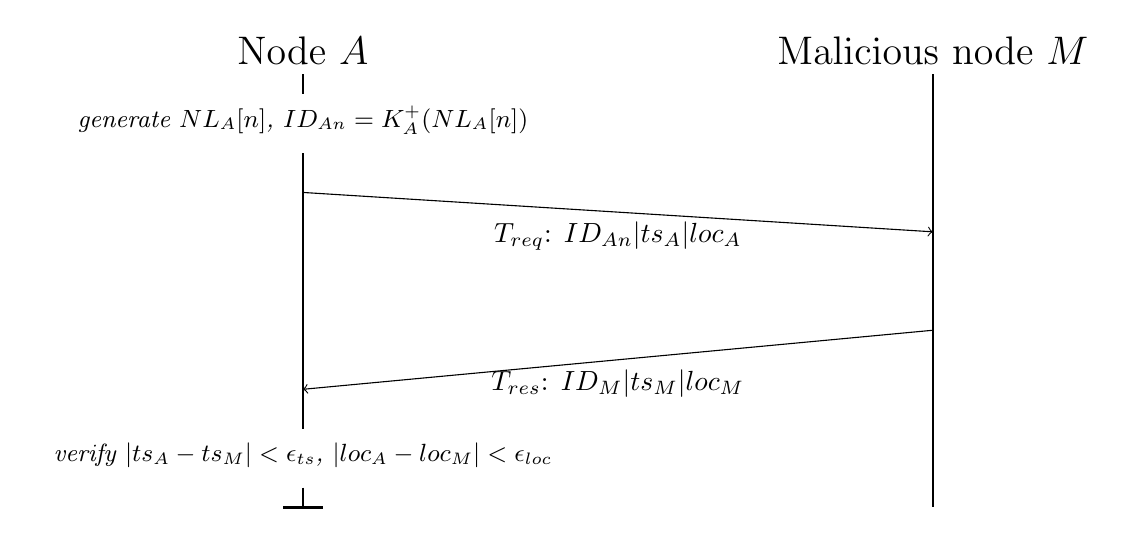
\begin{tikzpicture}
\coordinate (A_1) at (0,5.5);
\coordinate (A_2) at (0,5.25);
\coordinate (A_3) at (0,4.5);
\coordinate (A_8) at (0,1);
\coordinate (A_9) at (0,0.25);
\coordinate (A_12) at (0,0);
\coordinate (AF_L) at (-0.25,0);
\coordinate (AF_R) at (0.25,0);

\coordinate (B_1) at (8,5.5);
\coordinate (B_3) at (8,4.5);
\coordinate (B_8) at (8,3.25);
\coordinate (B_9) at (8,2.5);
\coordinate (B_12) at (8,0);

\draw[thick] (A_1)--(A_2) (A_3)--(A_8) (A_9)--(A_12) (AF_L)--(AF_R);
\draw[thick] (B_1)--(B_3) (B_3)--(B_9) (B_9)--(B_12);
\draw (A_1) node[above]{\Large Node $A$};
\draw (B_1) node[above]{\Large Malicious node $M$};

\draw (A_2) node[below,text centered]{\begin{tabular}{r}
\small{\textit{generate $NL_A[n]$, $ID_{An} = K^{+}_A(NL_A[n])$}}
\end{tabular}};

\coordinate (AX_1) at ($(A_3)-(0,0.5)$);
\coordinate (BX_1) at ($(B_3)-(0,1)$);
\draw[->] (AX_1) -- (BX_1) node[midway,below]
	{$T_{req}$: $ID_{An} | ts_A | loc_A$};

\coordinate (AX_2) at ($(A_3)-(0,3)$);
\coordinate (BX_2) at ($(B_8)-(0,1)$);
\draw[->] (BX_2) -- (AX_2) node[midway,below]
	{$T_{res}$: $ID_{M} | ts_M | loc_M$};
	
\draw (A_8) node[below,text centered]{\begin{tabular}{r}
\small{\textit{verify $|ts_A-ts_M| < \epsilon_{ts}$, $|loc_A-loc_M| < \epsilon_{loc}$}}
\end{tabular}};
\end{tikzpicture}}
\caption{An aborted transaction due to malicious node $M$}
\label{fig:aborted_transaction}
\end{figure}

\clearpage
\section{Verification} \label{ssec:verification}
In the verification stage, a mobile node tries to prove its location to a Verifier node, e.g. a bank. To do this, the mobile node sends the Verifier a number of parameters, as shown in Figure \ref{fig:verify_request}.

\begin{figure}[H]
\begin{center}
\resizebox {0.8\columnwidth} {!} {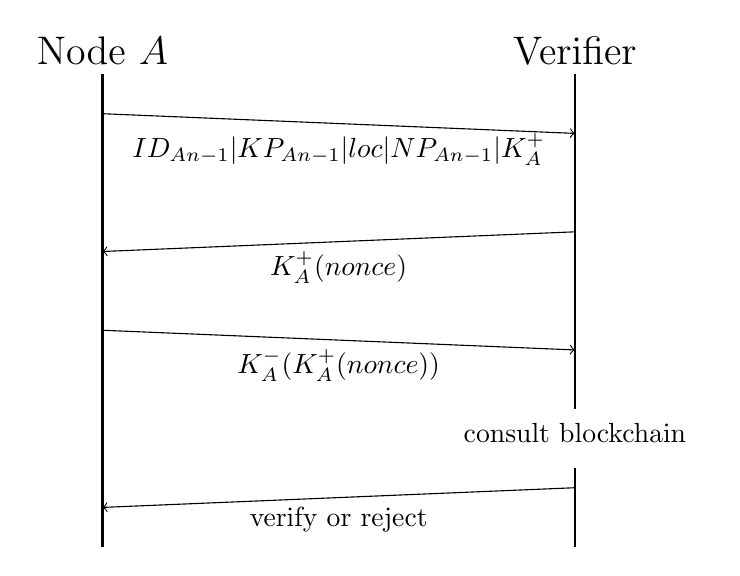
\begin{tikzpicture}
\coordinate (A_1) at (0,6);
\coordinate (A_2) at (0,0);

\coordinate (B_1) at (6,6);
\coordinate (B_2) at (6,1.75);
\coordinate (B_3) at (6,1);
\coordinate (B_4) at (6,0);

\draw[thick] (A_1)--(A_2);
\draw[thick] (B_1)--(B_2) (B_3)--(B_4);
\draw (A_1) node[above]{\Large Node $A$};
\draw (B_1) node[above]{\Large Verifier};

\coordinate (AX_1) at ($(A_1)-(0,0.5)$);
\coordinate (BX_1) at ($(B_1)-(0,0.75)$);
\draw[->] (AX_1) -- (BX_1) node[midway,below]
	{$ID_{An-1}|KP_{An-1}|loc|NP_{An-1}|K^{+}_A$};
	
\coordinate (AX_2) at ($(A_1)-(0,2.25)$);
\coordinate (BX_2) at ($(B_1)-(0,2)$);
\draw[->] (BX_2) -- (AX_2) node[midway,below]
	{$K^{+}_A(nonce)$};

\coordinate (AX_3) at ($(A_1)-(0,3.25)$);
\coordinate (BX_3) at ($(B_1)-(0,3.5)$);
\draw[->] (AX_3) -- (BX_3) node[midway,below]
	{$K^{-}_A(K^{+}_A(nonce))$};
	
\draw (B_2) node[below,text centered]{\begin{tabular}{r}
consult blockchain
\end{tabular}};

\coordinate (AX_2) at ($(A_1)-(0,5.5)$);
\coordinate (BX_2) at ($(B_1)-(0,5.25)$);
\draw[->] (BX_2) -- (AX_2) node[midway,below]
	{verify or reject};

\end{tikzpicture}}
\caption{Verification request}
\label{fig:verify_request}
\end{center}
\end{figure}

\begin{itemize}[noitemsep,topsep=0pt]
	\item[] $\mathbf{ID_{A}[n-1]}$ is the ID of $A$'s most recently published transaction.
	\item[] $\mathbf{KP_{An-1}}$ is $A$'s key packet up to transaction $n-1$, and includes keys for as many transactions as $A$ feels is appropriate in order to receive verification.
	\item[] $\mathbf{loc}$ is $A$'s current claimed GPS coordinates for which it is seeking verification.
	\item[] $\mathbf{NP_{An-1}}$ is $A$'s \textit{Nonce Packet}, a subset of its \textit{Nonce List} (section \ref{sssec:nonce_list}). A Nonce Packet is the list of the nonces used to generate $A$'s most recent IDs, up to $n-1$, that $A$ is willing to share with the Verifier. 
\end{itemize}

\null
The goal of the verification stage is for the Verifier to either accept or reject the location that the user is claiming. Given $ID_{A}[n-1]$ and $KP_{An-1}$, a Verifier is able to retrieve $A$'s previous transactions, and the transactions of all of its alibi's. This will allow the Verifier to recursively inspect the transactions of all alibi's used in a nodes transactions, until it is satisfied that the location can be verified or rejected. This recursive inspection can be visualised as a tree, as shown in figure \ref{fig:tree}.

\begin{figure}[H]
\begin{center}
\resizebox {0.7\columnwidth} {!} {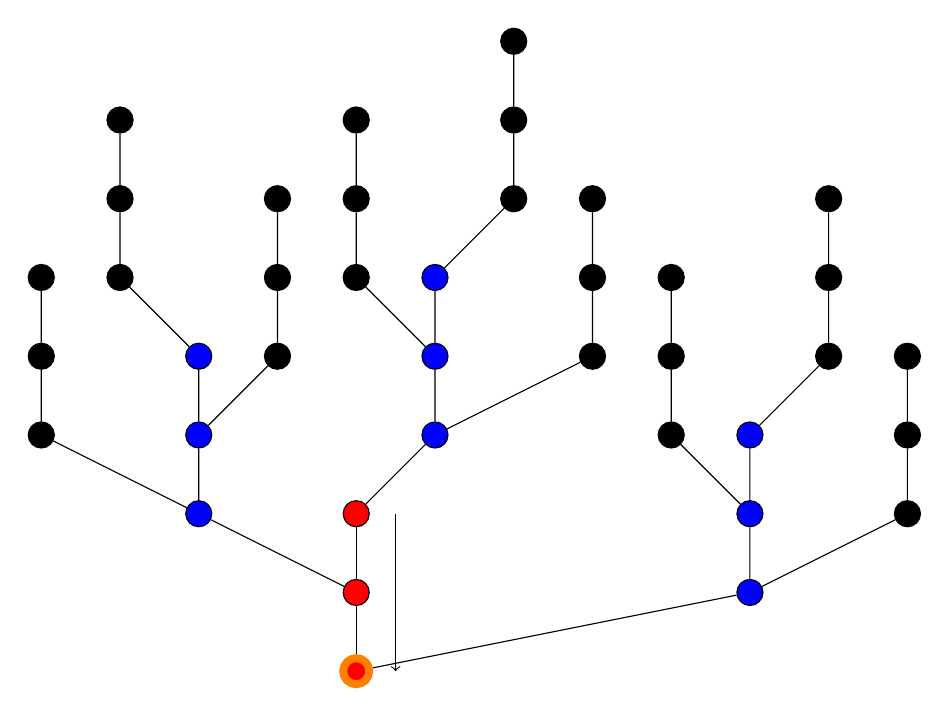
\begin{tikzpicture}[every node/.style={draw,shape=circle,fill=black}]

\node[fill=red,line width=1mm,draw=orange] (A) at (0,0) {};
\node[fill=red] (B) at (0,1) {};
\node[fill=red] (C) at (0,2) {};

\draw (A) -- (B) (B) -- (C);

\only<2> {
\draw[->] (0.5,2) -- (0.5,0);
}

\onslide<3->{
\node[fill=blue] (D) at (5,1) {};
\node[fill=blue] (E) at (5,2) {};
\node[fill=blue] (F) at (5,3) {};

\draw (A) -- (D) (D) -- (E) (E) -- (F);

\node[fill=blue] (G) at (-2,2) {};
\node[fill=blue] (H) at (-2,3) {};
\node[fill=blue] (I) at (-2,4) {};

\draw (B) -- (G) (G) -- (H) (H) -- (I);

\node[fill=blue] (J) at (1,3) {};
\node[fill=blue] (K) at (1,4) {};
\node[fill=blue] (L) at (1,5) {};

\draw (C) -- (J) (J) -- (K) (K) -- (L);
}

\onslide<4->{
\node (M) at (-4,3) {};
\node (N) at (-4,4) {};
\node (O) at (-4,5) {};

\draw (G) -- (M) (M) -- (N) (N) -- (O);

\node (P) at (-1,4) {};
\node (Q) at (-1,5) {};
\node (R) at (-1,6) {};

\draw (H) -- (P) (P) -- (Q) (Q) -- (R);

\node (S) at (-3,5) {};
\node (T) at (-3,6) {};
\node (U) at (-3,7) {};

\draw (I) -- (S) (S) -- (T) (T) -- (U);

\node (V) at (0,5) {};
\node (W) at (0,6) {};
\node (X) at (0,7) {};

\draw (K) -- (V) (V) -- (W) (W) -- (X);

\node (Y) at (2,6) {};
\node (Z) at (2,7) {};
\node (AA) at (2,8) {};

\draw (L) -- (Y) (Y) -- (Z) (Z) -- (AA);

\node (AB) at (3,4) {};
\node (AC) at (3,5) {};
\node (AD) at (3,6) {};

\draw (J) -- (AB) (AB) -- (AC) (AC) -- (AD);

\node (AE) at (4,3) {};
\node (AF) at (4,4) {};
\node (AG) at (4,5) {};

\draw (E) -- (AE) (AE) -- (AF) (AF) -- (AG);

\node (AH) at (6,4) {};
\node (AI) at (6,5) {};
\node (AJ) at (6,6) {};

\draw (F) -- (AH) (AH) -- (AI) (AI) -- (AJ);

\node (AK) at (7,2) {};
\node (AL) at (7,3) {};
\node (AM) at (7,4) {};

\draw (D) -- (AK) (AK) -- (AL) (AL) -- (AM);
}

\end{tikzpicture}}
\vspace{-3cm}
\caption{Alibi chain relationship tree}
\label{fig:tree}
\end{center}
\end{figure}

If the verifier wishes to recurse more, it could inspect the black node's alibis' transaction chains. Note that this is a simple example, and $n = 3$, the length of the transaction chain subset provided for verification. In reality $n$ should be much larger.

The Verifier uses $NP_{An-1}$ and $K^{+}_A$ to prove that node $A$ was the author of all of the transactions he claims to be. This prevents a collusion attack whereby nodes could share common transactions between different proof chains. When walking chronologically backwards along $A$'s proof chain, the 3rd party will ensure that the ID used in transaction $m$ on the proof chain matches $K^{+}_A(NP_{An-1}[m])$.

There are a huge number of possible factors involved in reaching a conclusion from the data on the blockchain; some of these factors will likely be unique to certain Verifiers, and kept secret to improve reliability and avoid gaming. Some simple example factors may include:
\begin{itemize}
	\item \textbf{Alibi credibility:} if each of the node’s alibi’s have little or no alibi’s themselves, they won't be considered credible alibis, and the Verifier will reject his verification request.
	\item \textbf{Transaction relevance:} if the Verifier considers the transactions it receives to be out of date, they will be rejected on the grounds that they are no longer relevant.
	\item \textbf{Alibi reuse:} if the Verifier can prove that alibi’s are being reused frequently, then it will reject the verification request.
	\begin{itemize}
		\item Due to transaction anonymity, the Verifier may not always be able to tell if two alibi's are the same person or not. e.g. node $A$ could use node $B$ as an alibi, then wait for $B$ to complete $n$ more transactions, then use node $B$ again.
		\item This is not a viable attack on the verification system. Depending on the size of $n$, enough time may pass between both uses of node $B$ as an alibi that the transactions are no longer relevant.
	\end{itemize}
\end{itemize}

\chapter{Evaluation}
The previous chapter introduced a model for a decentralised location proof system. This chapter will present an evaluation of the model with respect to the design goals defined in section \ref{sec:design_goals}.

\section{OTIT conformance}
As explained in section \ref{ssec:otit}, the OTIT model \cite{otit} defines 8 desirable properties of a lcoation proof system. The model introduced in chapter \ref{ch:design} is evaluated with respect to OTIT below.

\subsection{Chronological}
The chronological property of OTIT states that location proofs should be ordered according to the sequence of their creation.

This property is not enforced at the time of transaction publication in this system. This is to avoid revealing any transaction information to the miner nodes, therefore preserving the privacy of the transaction owner. Instead, the Chronological property is enforced at the time of verification. The chronological link created by adding $KL_{AT}(ID_{A}[n-1]|ts_A)$ to the published transaction will allow Verifier nodes to prove that the transaction is chronologically ordered. Therefore the system preserves OTIT's ``Chronological'' property.

\subsection{Order preserving}
This property states that the order in which location proofs were entered into the proof chain should be maintained.

In this system, a blockchain is used to store location proof transactions. In a blockchain, new blocks are added in a linear, chronological order, and cannot be modified so long as the majority of miners in the network are honest \cite{blueprint}.

A block consists of a number of transactions. These transactions are included in the block in the order they were received by the miner who solved the proof-of-work for that block. Once the block has been signed into the blockchain, it is impossible for the transactions inside the block to be reordered, assuming the miner network is controlled by a majority of honest nodes.

As a further method of preserving order, each node includes its observed timestamp in its encrypted transaction and link data. This prevents a group of malicious miner nodes from altering the order and timestamp of the transaction before signing it into the blockchain. Therefore the transactions stored in these blocks satisfy the ``Order preserving'' property of OTIT.

\subsection{Verifiable}
This states that a Verifier should be able to verify or reject the claim by the user that he has visited the given location(s).

The sytem described in chapter \ref{ch:design} inherently satisfies this property of OTIT. Verifier nodes may be operated by banks, employers, or other parties who have a vested interest in allowing their customers or employees to be able to prove their location. These Verifiers can verify or reject a mobile nodes claimed location by examining the nodes chronological link of transactions (as shown in figure \ref{fig:tree}). The Verifier will revursively generate and examine this tree until it can conclude whether the transaction chain is valid or not.

\subsection{Tamper evident}
The system is tamper evident, meaning the Verifier is able to detect if the proof chain has been tampered with or modified. If a malicious node creates a successful transaction with an honest node, but modifies the transaction data before publishing, a Verifier node will reject the malicious transaction. This rejection will be on the grounds that the matching transaction, published by the honest node, contains contradictory data.

The design assumes the underlying security of the blockchain, so any malicious miner nodes will not be able to tamper with existing transaction data providing that the majority of CPU power in the mining system is owned by honest miners \cite{bitcoin}. Therefore the tamper evident property is satisfied.

\subsection{Privacy preserved}
This property states that when the proof chain is verified for specific location proofs, privacy must be preserved for the other location proofs within the chain.

In the system, privacy is preserved using \textit{Key Lists} \ref{ssec:key_lists}. Two keys are used for each transaction; $KL_{AT}[n]$ is used to encrypt the \textit{transaction data} for $A$'s $nth$ transaction, and $KL_{AL}[n]$ is used to encrypt the \textit{backwards chronological link} between $A$'s $nth$ transaction and transaction $n-1$.

To control his privacy, a user can choose only to reveal $KL_{AL}[n]$ for a specific transaction $n$. This may be useful if a user does not wish to reveal transaction data for transactions created within a certain distance of his house, for example. Hiding $KL_{AT}[n]$ while revealing $KL_{AL}[n]$ has the advantage of preserving the user's privacy while maintaining a clear backwards chronological link of transactions for the Verifier to follow. This simulatneously preserves both privacy and chronological integrity.

\subsection{Selective in-sequence privacy}
This is the requirement that the user must be able to choose not to reveal certain location proofs within the proof chain when seeking verification. The system satisfies this property by using \textit{Key Packets} (section \ref{sssec:key_packets}).

A \textit{sub-set} of size $m$ of a node $A$'s proof chain, beginning at proof $n$, contains all proofs in the sequence $ID_{A}[n-m] - ID_{A}[n]$. Every transaction in this chain is split into two parts (a transaction data and link data part), and separately encrypted. If a node reveals keys for a verifier decrypt all transactions in the sequence $ID_{A}[n-m] - ID_{A}[n]$, it will not be possible for the verifier to discover transaction $ID_{A}[n-m-1]$, or any transaction outside the sequence $ID_{A}[n-m] - ID_{A}[n]$.

By encrypting each transaction with a different pair of keys, this system satisfies OTIT's ``selective in-sequence privacy'' property.

\subsection{Privacy protected chronology}
This property of OTIT states that the location proof system should ensure that the user does not hide important information from the items within the subset of the proof chain. In this system, it is impossible by design to hide important information, due to the use of backwards chronological linking between transactions. 

\subsection{Convenience and derivability}
This requirement states that the system must ensure that the user does not burden the Verifier with a large amount of data to analyse in order to verify the user's location.

In this system, the data is stored in a central blockchain that the Verifier has access to, and the user provides the Verifier  with decryption keys and indexes into just a sub-section of this data. Therefore the data sent to from the user to the Verifier, $KP_{An}$, is quite small in size.

The Verifier has the freedom to decide how comprehensively to investigate the users data; It can decide how far to recurse while investigating the tree of alibi relationships. This property of OTIT is therefore satisfied by allowing the Verifier to decide how complex the verification process needs to be.

\section{Threat analysis}
\subsection{False presence}
In a false presence attack, a dishonest user attempts to obtain a location proof for a false location.

In this system, any dishonest user attempting to obtain a location proof with an honest alibi will not succeed, as the honest alibi will abort the exchange (see section \ref{ssec:aborting_exchanges}). A dishonest user who publishes a transaction onto the blockchain with a fabricated alibi will also not succeed, as the transaction will be rejected during verification if a Verifier can't find the matching alibi transaction. The system is therefore not vulnerable to a false presence attack.

\subsection{Malicious intruders}
A malicious intruder offers to help another user to prove a false location, but doesn't prove a false location for himself.

In the context of this system, a malicious intruder may collude with another user to prove a false location, by acting as an alibi. These transactions will be successfully published onto the blockchain. However, if this user attempts to have his transaction chain verified, a Verifier will quickly notice the lack of credible alibis in the proof chain, indicating malicious activity, and reject the proof request. A sample tree of a node with uncredible alibis is shown in figure \ref{fig:uncredible_tree}. This avoids a malicious intruder vulnerability.

\begin{figure}[H]
\begin{center}
\resizebox {0.5\columnwidth} {!} {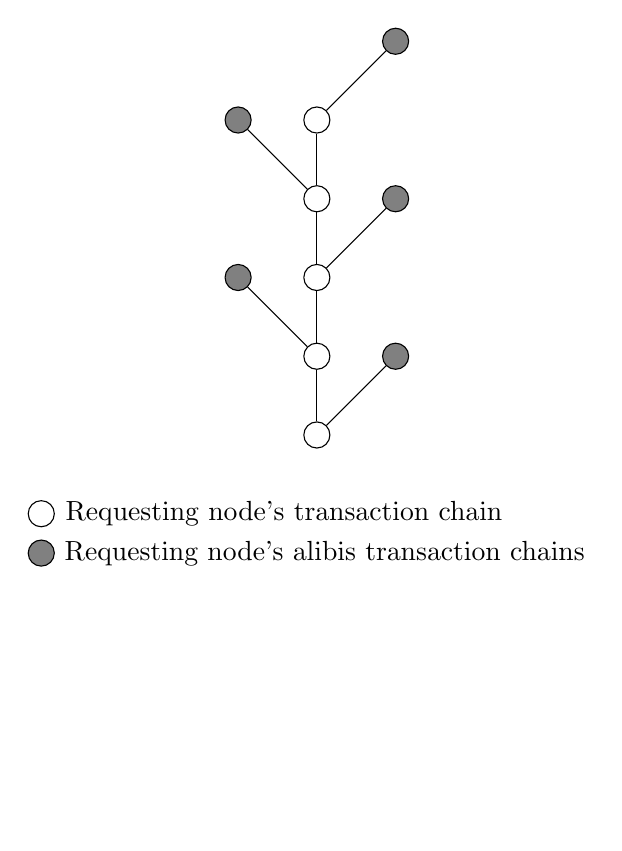
\begin{tikzpicture}[every node/.style={draw,shape=circle,fill=black}]

\node[fill=white] (A) at (0,0) {};
\node[fill=white] (B) at (0,1) {};
\node[fill=white] (C) at (0,2) {};
\node[fill=white] (D) at (0,3) {};
\node[fill=white] (E) at (0,4) {};

\node[fill=white,label=right:Requesting node's transaction chain] (L1) at (-3.5,-1) {};
\node[fill=gray,label=right:Requesting node's alibis transaction chains] (L2) at (-3.5,-1.5) {};

\draw (A) -- (B) (B) -- (C) (C) -- (D) (D) -- (E);

\node[fill=gray] (F) at (1,1) {};
\draw (A) -- (F);

\node[fill=gray] (G) at (-1,2) {};
\draw (B) -- (G);

\node[fill=gray] (H) at (1,3) {};
\draw (C) -- (H);

\node[fill=gray] (I) at (-1,4) {};
\draw (D) -- (I);

\node[fill=gray] (J) at (1,5) {};
\draw (E) -- (J);

\end{tikzpicture}}
\vspace{-3cm}
\caption{A proof chain with uncredible alibis}
\label{fig:uncredible_tree}
\end{center}
\end{figure}

\subsection{Curious users}
A curious user is one who learns another users identity by monitoring its location proofs.

Identity discovery is impossible by design in this sytem. By using a different, seemingly random identity for each transaction, it is impossible for a curious user to determine if two transactions belong to the same user or not. It is therefore impossible for a curious user to learn another users identity by monitoring location proofs.

\subsection{Malicious applications}
A malicious application is one that tries to take advantage of a users information as the user seeks verification.

This attack does not affect this system, as a user will only seek verification from applications (verifiers) it deems trustworthy. Verifiers, such as banks or employers, will be known to the user, and therefore trusted. The user also has complete control over which verifiers it chooses to seek verification from, it is not obliged to send verification requests to any verifier.

\subsection{Eavesdroppers}
An eavesdropper intercepts or modifies communication between two honest users. This threat does not affect this system, as ad-hoc bluetooth networks are set up between two mobile nodes advertising their current transaction ID, e.g. $ID_A[n]$. An eavesdropper will not be a member of this ad-hoc network, and therefore cannot modify any communication in the network.

\subsection{Wormhole attacks}
In a wormhole attack, an attacker records network traffic in one location and replays it in another location, at another time.

This attack is not relevant to the system presented in chapter \ref{ch:design}, as this system is decentralised. Any wormhole attack transmissions will simply be ignored by the intended victim.

\subsection{Weak identities}.
In a weak identity attack, a user gives his public key or identity to another colluding user in order to create a location proof.

A weak identity attack will not affect this system. Exchanging public keys or identities between colluding users offers no advantage. This is because the Verifier will ensure that any users requesting verification own the private key corresponding to the public key transferred during the verification request (see section \ref{ssec:verification}).

\subsection{False timestamping}
False timestamping includes backdating and future dating attacks. In a backdating attack, the attacker creates a location proof with a past timestamp. In future dating, the attacker creates a location proof with a future timestamp.

This system is resilient against a false timestamping attack by design. Every transaction is created with a reference to an alibi transaction. If an attacker creates a transaction with a past or future timestamp, the corresponding alibi transaction will contain contradictory information, and a Verifier will disregard it.

\subsection{Implication}
An implication attack occurs when a malicious user, or group of colluding malicious users, create a false location proof for an honest user.

This system is resilient to an implication attack. Location proofs are stored in a public blockchain, but the decryption keys, nonce and public key used to create the transaction all reside with the user who created it. A user cannot be implicated in a location proof without creating the identity used in the proof, and encrypting the transaction data.

It is therefore impossible to implicate an honest user in a location proof, without finding vulnerabilities outside the location proof system (for example by compromising their device).

\subsection{False assertion}
In a false assertion attack, two malicious users collude to create false location proofs for themselves.

It is possible in this system for two malicious users to collude as alibis and publish their transactions on the blockchain. This is allowed because the miner nodes do not know the contents of the data they are signing into the blockchain, as it is encrypted.

Providing that the system is comprised of a majority of honest nodes, this attack will not succeed. It will be obvious to a Verifier after construcing a graph of the nodes alibi transaction (as shown in section \ref{ssec:verification}) that the graph lacks alibi credibility, and therefore two malicious users are likely colluding to create location proofs for themselves. Therefore the system is not vulnerable to this attack.

\subsection{Proof switching}
In a proof switching attack, a malicious user modifies one of its existing honest proofs to spoof a false location.

This is not possible in this system, as the blockchain is used as a tamper-proof method of storing location proofs. Once the proof is included in the blockchain, it cannot be modified.

If the proof has not been added to the blockchain yet, then it is possible for the malicous user to modify it to attempt to spoof a false location. However this attack will not work on this system. Any Verifier will reject the transaction on the grounds that it contains contradictory information to the alibis transaction, which has not been modified.

\subsection{Relay attack}
In a relay attack, a malicious user uses a colluding \textit{proxy user} physically present at the location that the malicious user wishes to create a false proof, to create a location proof with an honest user.

This system is resilient against a most relay attacks. This is because proofs created using a proxy user will be inconsistent with the other proofs in a users proof chain. For example, a user living in New York uses a proxy user to create a proof with a user in London. A Verifier will reject the users claim that it is in London, because of the lack of alibi credibility.

One vulnerability of the system can be called a \textit{complete} relay attack. In a \textit{complete} relay attack, two malicious nodes exist purely for the purpose of proxying location proof. One node, the proxy, will \textit{never} request location proofs for itself. Its only purpose is to proxy exchange data between honest nodes and the other malicious node, the \textit{attacker}.

Resilience against a complete relay attack scenario must be taken out of the scope of this system. 

\subsection{Sybil attack}
A Sybil attack occurs when a single malicious user generates multiple \textit{pseudoidentities}, and begins masquerading as multiple users.

While some studies have been done on Sybil attacks in decentralised systems \cite{sybil}. There are various methods of mitigating against a subil attack, however a solution for the Sybil attack in a decentralised system is considered an open problem. This system is therefore vulnerable to a highly targeted Sybil attack.



\chapter{Future work}

\newpage
\begin{thebibliography}{9}

\bibitem{brassil}
  J. Brassil, P.K. Manadhata,
  ``Verifying the Location of a Mobile Device User'',
  Proc. of MobiSec 2012,
  June 2012.

\bibitem{luo}
  W. Luo, U. Hengartner,
  ``Proving your Location without giving up your Privacy'',
  Proceedings of the Eleventh Workshop on Mobile Computing Systems \& Applications,
  HotMobile 2010, Annapolis, Maryland, February 22 - 23, pp. 7–12. ACM,
  New York (2010).

\bibitem{khan}
  R. Khan, S. Zawoad, M. Haque, and R. Hasan,
  ```Who, When, and Where?' Location Proof Assertion for Mobile Devices'',
  Proceedings of the 28th Annual IFIP WG 11.3 Working Conference on Data and Applications Security and Privacy, ser. DBSec. IFIP,
  July 2014.
 
\bibitem{otit}
  R. Khan, S. Zawoad, M. Haque, and R, Hasan.
  ``OTIT: Towards secure provenance modeling for location proofs'',
  Proc. of ASIACCS. ACM (2014).

\bibitem{sybil}
  J.R. Douceur,
  ``The sybil attack'',
  Druschel, P., Kaashoek, M.F., Rowstron, A. (eds.) IPTPS 2002. LNCS, vol. 2429, pp. 251–260,
  Springer, Heidelberg (2002).

\bibitem{maxmind}
  MaxMind LLC. GeoIP. http://www.maxmind.com,
  2010.

\bibitem{constraint-based}
  B. Gueye, A. Ziviani, M. Crovella, and S. Fdida,
  ``Constraint-based geolocation of Internet hosts'',
  IEEE/ACM Transactions on Networking,
  14(6):1219–1232, 2006.

\bibitem{location-spoof}
  N. O. Tippenhauer, K. B. Rasmussen, C. Popper, and S. Capkun,
  ``iPhone and iPod location spoofing: Attacks on public WLAN-based positioning systems'',
  SysSec Technical Report,
  ETH Zurich, April, 2008.

\bibitem{tor}
  R. Dingledine, N. Mathewson, and P. Syverson,
  ``TOR: The second generation onion router'',
  Proceedings of the Usenix Security Symposium,
  2004.

\bibitem{distributed}
  G. Coulouris, J. Dollimore, T. Kindberg, and G. Blair,
  ``Distributed Systems: Concepts and Design (5th Edition)'',
  Boston: Addison-Wesley,
  2011.

\bibitem{blueprint}
  M. Swan,
  ``Blockchain: Blueprint for a New Economy'',
  Sebastopol, CA,
  O’Reilly Media, 2015

\bibitem{bitcoin}
  S. Nakamoto,
  ``Bitcoin: A Peer-to-Peer Electronic Cash System'',
  2008
  
\bibitem{femtocell}
  V. Chandrasekhar, J. Andrews, and A. Gatherer,
  ``Femtocell Networks: A Survey'',
  IEEE Communications Magazine, Vol. 46, No. 9, pps. 59-67,
  September 2008
  
\bibitem{ddos}
  J. Mirkovic, P. Reiher,
  ``A taxonomy of DDoS attack and DDoS defense mechanisms'',
  ACM SIGCOMM Comput. Commun. Rev. 34, 2, 39–53,
  2004

\end{thebibliography}

\end{document}